
\section{The Shared Manifold Hypothesis}
\label{sec:prior}

Having established the existence of transfer learning from LLMs to time series in Sec.~\ref{sec:transfer}, we now present a geometric explanation for why LLMs are such adept time series forecasters. Due to the recursive structure and statistical patterns exhibited by language \citep{ou2025identifying}, we theorize that pretrained language model representations already contain native temporal structures well suited for adaptation to time series data. In this section, we present several experiments demonstrating that LLMs do possess a manifold that is already compatible with time series forecasting, and that fine-tuning does not need to create new directions, it simply identifies and collapses time series representations onto the best pre-existing directions.

\subsection{A Linear Probe Reveals Latent Temporal Structure}
% ── FIGURE: Examples + Ablation side by side ──
\begin{figure}[!t]
\centering
\begin{subfigure}[t]{0.48\textwidth}
\centering
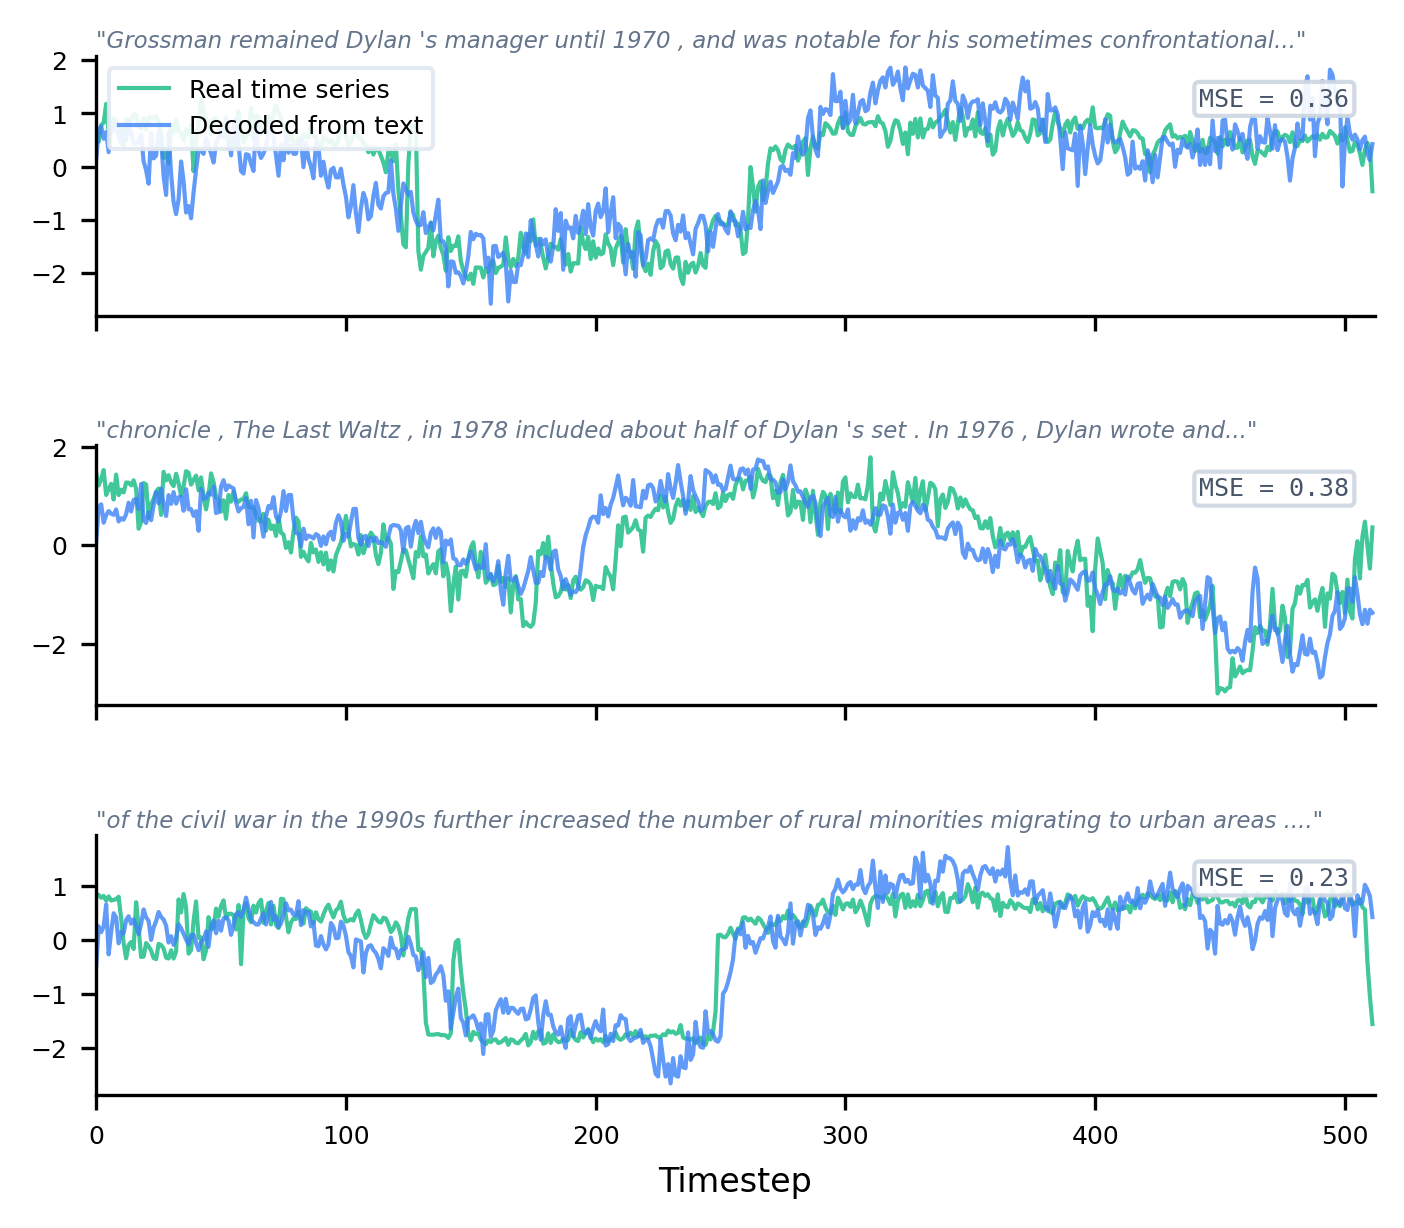
\includegraphics[width=\textwidth]{figures/sec4/panel_b_examples.png}
\caption{Decoded time series from text}
\label{fig:examples}
\end{subfigure}
\hfill
\begin{subfigure}[t]{0.48\textwidth}
\centering
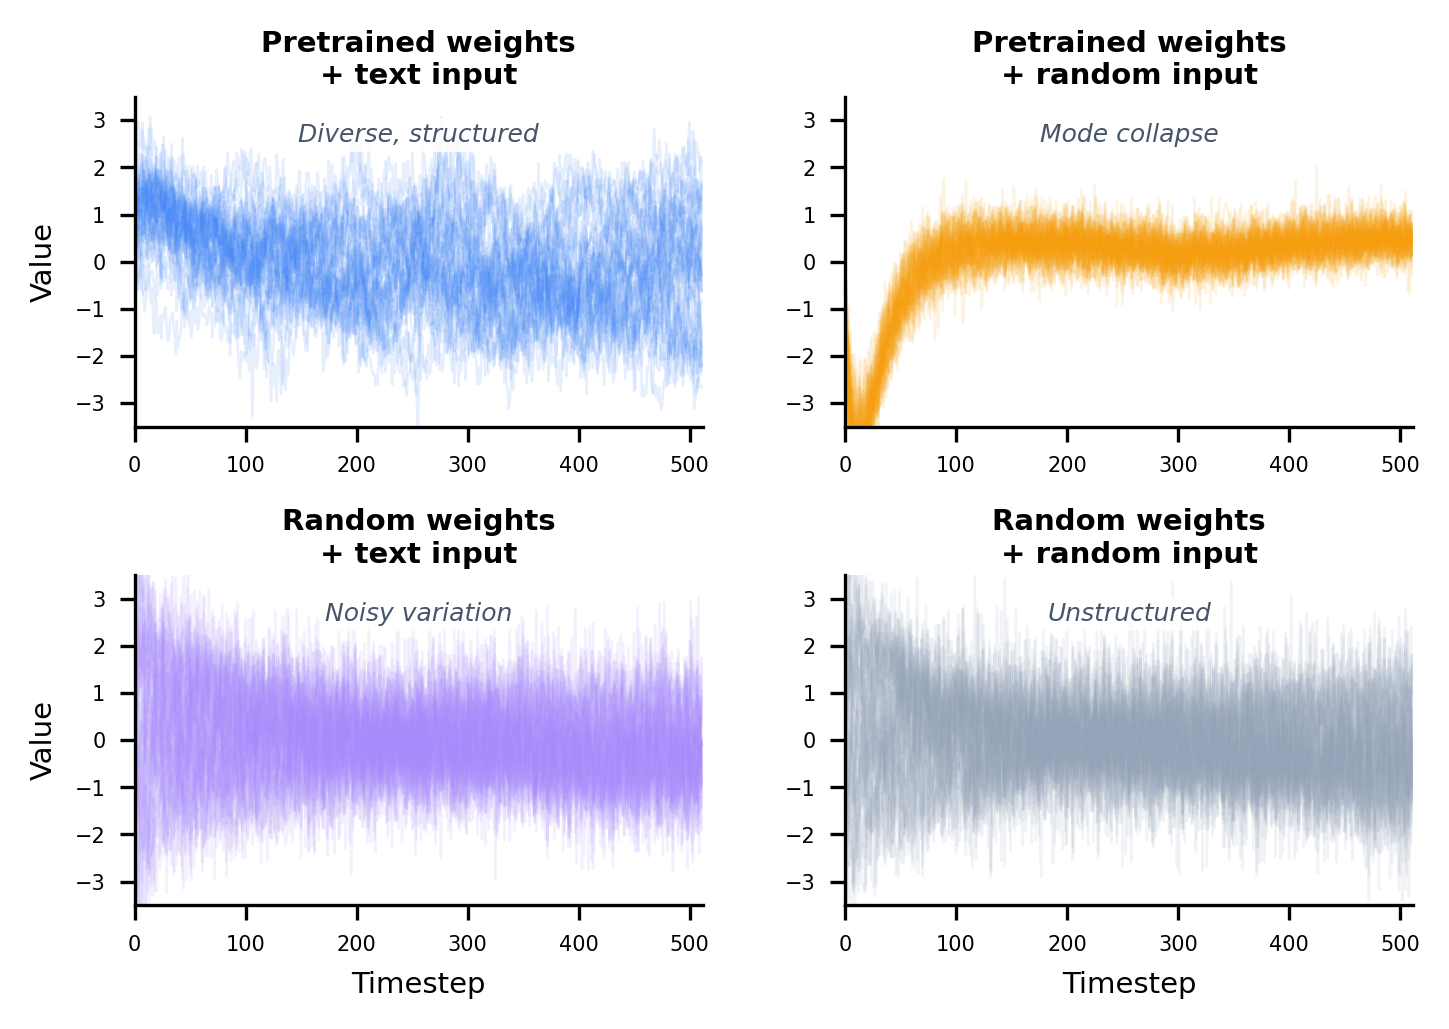
\includegraphics[width=\textwidth]{figures/sec4/panel_c_ablation.png}
\caption{Ablation: what creates the structure?}
\label{fig:ablation}
\end{subfigure}
\caption{\textbf{Pretrained hidden states contain time-series-compatible structure.} A single linear map $\hat{y}_t = \mathbf{w}^\top \mathbf{h}_t + b$ is trained on frozen LLM hidden states via EM-style nearest-neighbor matching to a bank of 10{,}000 real time series (no paired data). \textbf{(a)} Three decoded outputs (blue) overlaid with their nearest real time series (green). Input text shown above each plot. MSE $= 0.23$--$0.38$; full distribution in Appendix. \textbf{(b)} Ablation crossing learned weights vs.\ random init with text vs.\ random input. \emph{Top-left}: pretrained + text---diverse, structured outputs (301 unique matches). \emph{Top-right}: pretrained + random tokens---mode collapse to one shape (manifold exists but is not traversed). \emph{Bottom-left}: random weights + text---noisy variation without structure. \emph{Bottom-right}: random weights + random tokens---unstructured. Only pretrained weights \emph{and} meaningful text together produce diverse temporal signals.}
\label{fig:hero}
\end{figure}

\label{sec:linear_decoding}
 In these experiments, we learn an linear mapping, $\hat{y}_i \in \R^T$, provided in Eq.~\ref{eq:linear_map}, from a frozen, pre-trained language model's hidden states. For each WikiText sequence, hidden states are extracted from all 28 layers and concatenated per timestep, $\mathbf{h}_{i,t} = [\mathbf{h}_{i,t}^{(0)}; \ldots; \mathbf{h}_{i,t}^{(27)}] \in \R^{D}$, where $D$ is $28{,}672$. The per-timestep linear map then produces a predicted sequence that is z-normalized to zero mean and unit variance. Using an EM-style nearest-neighbor algorithm, each prediction is matched with its closest time series from GiftEval. Fig.~\ref{fig:ablation}(a) shows plots of three of these predictions (blue) along with their closest GiftEval matches (green), on a set of data not included in the training of the linear layer. The mapping is optimized to minimize MSE to these assignments, with a spectral diversity penalty, $\lambda$, to prevent collapse.
  \begin{equation}
 \label{eq:linear_map}
     \hat{y}_{i,t} = \mathbf{w}^\top \mathbf{h}_{i,t} + b
 \end{equation}
  
Out of $1920$ wiki text samples, the linear map produces $686$ unique matches to one of the $10{,}000$ real time series. The map generalizes to $439$ unique held-out WikiText text sequences out of $1000$, strongly suggesting that the pre-trained language model's representation space already contains directions whose projections resemble temporal signals.
 
The fact that linear probing can extract realistic time-series from language model hidden states has direct implications for fine-tuning these language models to predict time-series. Let $\mathcal{M} \subset \R^D$ denote the manifold of hidden-state trajectories produced by the pre-trained language model processing text. The experiments demonstrate the existence of a direction $\mathbf{w} \in \R^D$ such that the distribution of projected trajectories, $\{\mathbf{w}^\top \mathbf{h}_t\}_{t=1}^T$ has significant overlap with the distribution of real time series, $P_{\mathrm{TS}}$. If we define $\mathbf{h}*t$ as the hidden state of the pretrained model %at timestep $t$, 
due to its autoregressive training, the model implements a deterministic update shown in Eq.~\ref{eq:deterministic_update} and learns to predict $x_{t+1}$ from $\mathbf{h}_t$. In practice, this means that the model has learned structured dynamics over the hidden states and given $\mathbf{h}*t$, it can reliably produce the next state $\mathbf{h}*{t+1}$ along trajectories induced by natural text.

\begin{equation}
\label{eq:deterministic_update}
    \mathbf{h}_{t+1} = F(\mathbf{h}*t, x*{t+1})
\end{equation}

The linear probing experiments demonstrate that a projection direction, $\mathbf{w}$, resembling a real-world time series can indeed be found within the frozen language models representation space. Because the LLM is trained to predict the next token $x_{t+1}$ by evolving its internal state, the function $F$ in Eq.~\ref{eq:deterministic_update} acts as a latent dynamical system for the temporal manifold. The model must implicitly predict $\mathbf{h}_{t+1}$ to make autoregressive predictions so it already possess the ability to propagate these signals through time. Once obtained, $\mathbf{h}*{t+1}$ can be combined with the pre-existing direction $\mathbf{w}$ and applied to Eq.~\ref{eq:linear_map} to produce $y_{t+1} = \mathbf{w}^\top \mathbf{h}_{t+1}$. This confirms that the pre-trained language model ca propagate hidden states along trajectories consistent with real-world time series.

In summary, fine-tuning language models for time series does not require learning the dynamics from scratch, it is a low-dimensional alignment problem that requires selecting and scaling existing directions in representation space.

\subsection{this needs a new section or appendix relocation}
The latent temporal structure exhibited above could have a variety of explanations which we attempt to 
%transformer architectures possess residual connections that produce smooth trajectories, the learned weights (pretraining compresses representations), or the input (natural text has sequential structure). 
disentangle by crossing model weights (pretrained vs.\ randomly initialized, same architecture) with input (WikiText vs.\ random tokens). A clear interaction emerges, \textit{pre-trained weights} create a structured, low-dimensional manifold, but random tokens fail to traverse it, Tab.~\ref{tab:ablation} shows that \textit{rand+PT} collapses to just four unique outputs. \textit{Meaningful text} provides variation, but without pretrained weights, this variation is unstructured noise (Tab.~\ref{tab:ablation} \textit{text+RandInit}). Only the combination produces diverse, high-quality temporal signals. In this case, the pretrained manifold provides the geometry, and text input drives its diverse traversal.

\begin{table}[h]
\centering
\caption{$2\times 2$ ablation. \emph{Unique}: distinct real TS matched. \emph{NN}: mean nearest-neighbor MSE. Low NN with low Unique indicates mode collapse, not quality. We need to fix the NN because its not normalized by the number of matches}
\label{tab:ablation}
\begin{tabular}{lrrrr}
\toprule
Condition & Train Unique & Held-Out Unique & Held-Out NN & Clusters \\
\midrule
\textbf{text + PT}   & \textbf{686}/1920 & \textbf{439}/1000 & 0.717 & 14/20 \\
text + RandInit       & 54/1920           & 73/1000            & 0.541 & 13/20 \\
rand + PT             & 4/1920            & 1/1000             & 0.293 & 4/20  \\
rand + RandInit       & 99/1920           & 138/1000           & 0.741 & 14/20 \\
\bottomrule
\end{tabular}
\end{table}


\subsection{The Projected Dynamics Forecast Beyond the Context}
\label{sec:forecasting}

The linear decoding result shows shape-level similarity between projected hidden states and real time series. We test whether this extends to \emph{predictive} structure: given the first half of a time series, can a retrieved text projection forecast the second half?

\paragraph{Method.} We take 500 real time series from GiftEval and observe only the first 256 of 512 timesteps. Among 10{,}000 WikiText projections, we retrieve the one with lowest MSE on the observed first half and use that projections second half as the forecast. The baseline is last-value carry-forward \textit{i.e.} repeating the final observed value.

\paragraph{Result.} Across all 500 queries, the retrieval-based forecast achieves MSE $= 1.91$ versus last-values $2.27$ ($16\%$ lower). The retrieval wins in $37\%$ of cases; when it wins, the advantage is large (median $4\times$ lower MSE), because the retrieved projection captures trends and level shifts that last-value misses entirely. Figure~\ref{fig:forecasting} shows the best-case example from our evaluation set.

\begin{figure}[h]
\centering
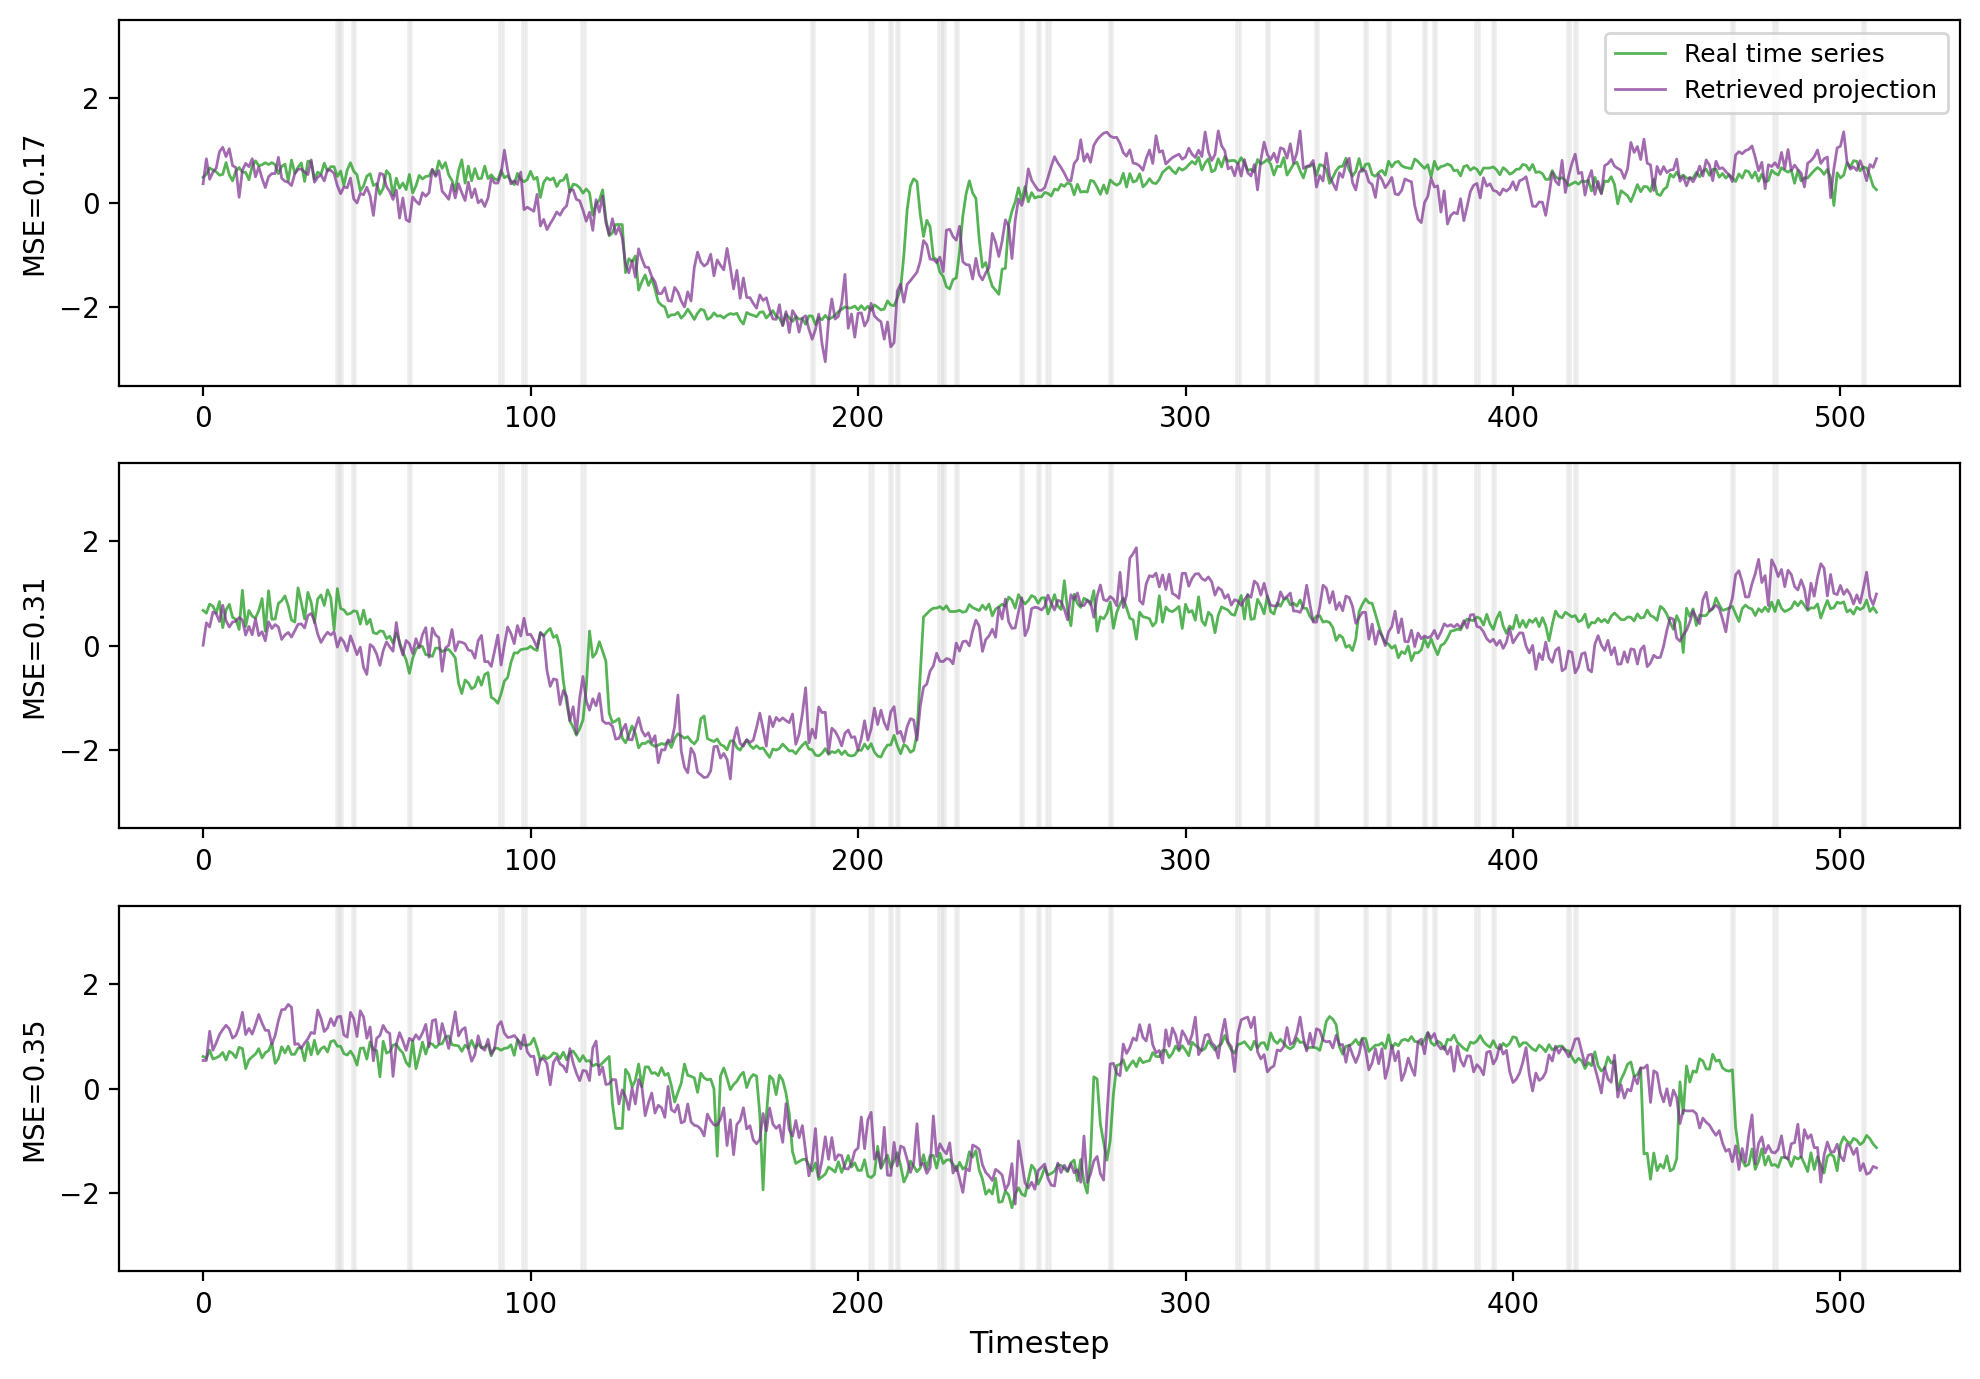
\includegraphics[width=\textwidth]{figures/sec4/panel_forecasting.png}
\caption{Forecasting example with largest gap compared to baseline from 500 evaluation queries. The first 256 timesteps are used to retrieve the closest WikiText projection; the projection's second half (purple) forecasts the continuation. The retrieved projection captures the level shift and subsequent trend (MSE $= 0.42$), while last-value carry-forward (gray dashed) is stranded at the final context value (MSE $= 11.7$).}
\label{fig:forecasting}
\end{figure}


\subsection{Pretraining Creates Coherent Gradient Signal for the TS Objective}
\label{sec:curvature}

\begin{figure}[h]
\centering
\includegraphics[width=\textwidth]{figures/sec4/fig_headline_7.png}
\caption{.}
\label{fig:grad_alignment}
\end{figure}

\textbf{details in the md file https://hackmd.io/VIS4nmT6Q2ms66mMUXTgWQ}

The manifold structure has direct consequences for optimization. We compute per-example gradients of the TS loss at the pretrained versus random initialization, measuring whether individual training examples provide coherent or contradictory optimization signals.

\paragraph{Method.} For 30 individual TS sequences, we compute the gradient $\mathbf{g}_i = \nabla_\theta L_i$ restricted to layers 6--10 (78.7M parameters) at both initializations. We measure pairwise cosine similarity $\cos(\mathbf{g}_i, \mathbf{g}_j)$ across all example pairs, and the signal-to-noise ratio $\mathrm{SNR} = \|\bar{\mathbf{g}}\| / \mathrm{mean}(\|\mathbf{g}_i - \bar{\mathbf{g}}\|)$.

\begin{table}[h]
\centering
\caption{Per-example gradient structure at the TS loss surface. At PT initialization, different TS examples produce gradients that reinforce each other. At random initialization, gradients are nearly orthogonal and cancel upon averaging.}
\label{tab:gradient_alignment}
\small
\begin{tabular}{lcc}
\toprule
Metric & PT init & Random init \\
\midrule
Per-example gradient cosine & \textbf{0.58} & 0.04 \\
Gradient signal-to-noise ratio & \textbf{1.16} & 0.28 \\
Gradient norm (RMS) & 0.0040 & 0.0004 \\
\bottomrule
\end{tabular}
\end{table}

\paragraph{Interpretation.} At PT initialization, per-example TS gradients have cosine similarity 0.58---different time series sequences agree on which direction to adjust the weights. Batch averaging reinforces this shared signal. At random initialization, gradients are nearly orthogonal (cosine 0.04, consistent with random vectors in $\sim$78M dimensions), so averaging causes massive cancellation: the SNR drops to 0.28, meaning most of the per-example gradient signal is lost.

This coherence arises because the pretrained representations create consistent feature activations across different TS inputs. When the loss asks ``how should this weight change?'', the answer is similar regardless of which TS sequence is used, because the pretrained features impose a shared structure on the loss landscape. At random initialization, each example activates arbitrary features, giving contradictory signals.

The effect is layer-dependent: gradient norms at PT initialization are 3--19$\times$ larger than at random initialization, with the ratio increasing for deeper layers (where random weights scramble the signal most). This layer-wise gradient structure explains why mid-to-deep layers benefit most from pretrained initialization (Section~\ref{sec:dimensionality}).

% Rerun this and the above across multiple checkpoints
\paragraph{Curvature anisotropy.} To characterize the \emph{shape} of the loss landscape, we compute the curvature $\mathbf{v}^\top H \mathbf{v}$ along 200 random unit vectors $\mathbf{v}$ in layers 6--10 parameter space using exact Hessian-vector products (Pearlmutter trick), and compare this to the curvature along the gradient direction $\hat{\mathbf{g}}$. At PT initialization, the gradient direction has curvature $232$, while the mean curvature across random directions is $9.6 \times 10^{-5}$---a ratio of $2.4 \times 10^6$. At random initialization, the gradient direction has curvature $-0.08$ (near-zero, slightly negative), barely distinguishable from random directions (mean $8.4 \times 10^{-7}$, ratio $\sim$80$\times$). The PT landscape is thus \emph{massively anisotropic}: SGD's natural descent direction is aligned with one of the very few high-curvature directions in a $\sim$78M-dimensional space, while the vast majority of directions are flat. At random initialization, the landscape is nearly isotropic---all directions, including the gradient, have negligible curvature.